\documentclass[12pt,a4paper]{article}

% ====== ENCODING & IDIOMA ======
\usepackage[utf8]{inputenc}   % entrada UTF-8
\usepackage[T1]{fontenc}      % output con font T1 (acentos correctos)
\usepackage[spanish]{babel}   % idioma español (división silábica, títulos, etc.)


% ====== DISEÑO DE PÁGINA ======
\usepackage{geometry}
\geometry{margin=1in}
\usepackage{setspace}
\onehalfspacing
\usepackage{parskip} % mejor separación entre párrafos
\usepackage{fancyhdr}
\usepackage{titlesec}

% ====== GRÁFICOS, TABLAS, CÓDIGO ======
\usepackage{graphicx}
\usepackage{float}       % [H] para fijar figuras/tablas
\usepackage{booktabs}    % tablas bonitas
\usepackage{caption}
\usepackage{xcolor}
\usepackage{listings}    % bloques de código simples
\lstset{
  basicstyle=\ttfamily\small,
  breaklines=true,
  frame=single,
  columns=fullflexible,
  showstringspaces=false
}
\usepackage{amsmath}

% (Opcional) Si quieres hipervínculos en el PDF
\usepackage[hidelinks]{hyperref}

% ====== ENCABEZADO/PIE ======
\pagestyle{fancy}
\fancyhf{}
\fancyhead[L]{IC-6600 Principios de Sistemas Operativos}
\fancyhead[R]{II Semestre 2025}
\fancyfoot[C]{\thepage}

% ====== FORMATO DE SECCIONES ======
\titleformat{\section}{\large\bfseries}{\thesection.}{0.5em}{}
\titleformat{\subsection}{\normalsize\bfseries}{\thesubsection.}{0.5em}{}

% ====== RUTAS DE IMÁGENES ======
% Ajusta si tus figuras están en otra carpeta:
\graphicspath{{./}{./bench/}}

% ====== DOCUMENTO ======
\begin{document}

% -------- PORTADA --------
\begin{titlepage}
    \centering
    
\includegraphics[width=0.5\textwidth]{img/logo-tec.png}
    \vspace{1cm}

    {\LARGE Instituto Tecnológico de Costa Rica \par}
    \vspace{0.5cm}
    {\Large Escuela de Ingeniería en Computación \par}
    \vspace{0.5cm}

    {\LARGE \textbf{IC-6600 Principios de Sistemas Operativos}}\\[2cm]

    {\huge \textbf{Tarea 03: Administración de Memoria}}\\[3cm]

    \textbf{Estudiantes:}\\[0.3cm]
    Anthony Barrantes Jimenez -- 2023152240\\
    Samir Fernando Cabrera Tabash -- 2022161229\\
    Deyton Hernandez Cordoba -- 2023036696\\[1.5cm]

    \textbf{Profesor:}\\[0.3cm]
    Kenneth Roberto Obando Rodríguez\\[1cm]

    16 de noviembre de 2025 \\[0.3cm]
    II Semestre 2025
    \vfill
\end{titlepage}

% -------- ÍNDICE (opcional) --------
 \tableofcontents
 \newpage

% -------- INTRODUCCIÓN --------
\section{Introducción}

Este documento presenta la implementación de un simulador de gestión dinámica de memoria en lenguaje C, desarrollado como parte de la Tarea 3 del curso IC-6600 Principios de Sistemas Operativos. El simulador replica el comportamiento de las funciones estándar de memoria dinámica (\texttt{malloc}, \texttt{calloc}, \texttt{realloc} y \texttt{free}) operando sobre un único bloque de memoria preasignado.

El objetivo principal del proyecto es demostrar el funcionamiento interno de la administración de memoria, incluyendo la implementación de tres estrategias clásicas de asignación (First-Fit, Best-Fit y Worst-Fit), así como la simulación de problemas comunes como la fragmentación externa y las fugas de memoria.

\subsection{Objetivos del Proyecto}

\begin{itemize}
    \item Implementar un gestor de memoria que opere sobre un pool de bytes preasignado.
    \item Desarrollar tres algoritmos de asignación de memoria: First-Fit, Best-Fit y Worst-Fit.
    \item Simular operaciones de asignación (\texttt{ALLOC}), reasignación (\texttt{REALLOC}) y liberación (\texttt{FREE}) de memoria.
    \item Demostrar problemas de fragmentación de memoria y fugas de memoria.
    \item Implementar expansión dinámica del pool de memoria utilizando \texttt{realloc}.
\end{itemize}

% -------- ARQUITECTURA DEL SISTEMA --------
\section{Arquitectura del Sistema}

El simulador está organizado en módulos independientes que facilitan el mantenimiento y la escalabilidad del código. La estructura de directorios del proyecto es la siguiente:

\begin{lstlisting}[language=bash]
Code/
├── src/          # Archivos fuente (.c)
│   ├── main.c
│   ├── memsim.c
│   ├── block.c
│   ├── varmap.c
│   └── util.c
├── include/      # Archivos de cabecera (.h)
│   ├── memsim.h
│   ├── block.h
│   ├── varmap.h
│   └── util.h
├── build/        # Archivos objeto (.o)
├── Makefile      # Sistema de compilación
└── entrada.txt   # Archivo de prueba
\end{lstlisting}

\subsection{Módulos del Sistema}

\subsubsection{main.c - Punto de Entrada}

El módulo principal se encarga de:
\begin{itemize}
    \item Validar los argumentos de línea de comandos (estrategia, tamaño del pool, archivo de entrada).
    \item Inicializar la estructura del simulador de memoria.
    \item Invocar el procesamiento del script de operaciones.
    \item Liberar todos los recursos al finalizar.
\end{itemize}

\subsubsection{memsim.c - Motor del Simulador}

Contiene la lógica principal del simulador:
\begin{itemize}
    \item \textbf{Inicialización}: Asigna el pool de memoria inicial usando \texttt{calloc}.
    \item \textbf{Expansión}: Implementa crecimiento dinámico del pool con \texttt{realloc}.
    \item \textbf{Estrategias de asignación}: Implementa First-Fit, Best-Fit y Worst-Fit.
    \item \textbf{Operaciones de memoria}: \texttt{do\_alloc}, \texttt{do\_realloc}, \texttt{do\_free}.
    \item \textbf{Visualización}: Función \texttt{print\_state} para mostrar el estado de la memoria.
    \item \textbf{Parser}: Procesa el archivo de entrada línea por línea.
\end{itemize}

\subsubsection{block.c - Gestión de Bloques}

Maneja la lista doblemente enlazada de bloques de memoria:
\begin{itemize}
    \item Creación de nuevos bloques (\texttt{new\_block}).
    \item Inserción y eliminación de bloques en la lista.
    \item Coalescencia de bloques libres adyacentes (\texttt{try\_coalesce}).
\end{itemize}

\subsubsection{varmap.c - Mapeo de Variables}

Implementa un diccionario simple que asocia nombres de variables con sus bloques de memoria:
\begin{itemize}
    \item Búsqueda de variables (\texttt{find\_var}).
    \item Registro de nuevas variables (\texttt{set\_var}).
    \item Eliminación de variables (\texttt{unset\_var}).
\end{itemize}

\subsubsection{util.c - Utilidades Generales}

Funciones auxiliares del sistema:
\begin{itemize}
    \item Manejo de errores (\texttt{die}).
    \item Asignación de memoria con verificación (\texttt{xmalloc}, \texttt{xstrdup}).
    \item Parseo de estrategias desde cadenas de texto.
\end{itemize}

% -------- ESTRUCTURAS DE DATOS --------
\section{Estructuras de Datos}

\subsection{BlockHeader - Descriptor de Bloque}

Cada bloque de memoria (libre u ocupado) está representado por la siguiente estructura:

\begin{lstlisting}[language=C]
typedef struct BlockHeader {
    size_t offset;           // Posición en el pool
    size_t size;             // Tamaño del bloque
    int free;                // 1 = libre, 0 = ocupado
    struct BlockHeader *prev; // Bloque anterior
    struct BlockHeader *next; // Bloque siguiente
} BlockHeader;
\end{lstlisting}

Esta lista doblemente enlazada permite:
\begin{itemize}
    \item Recorridos eficientes en ambas direcciones.
    \item Coalescencia rápida de bloques adyacentes.
    \item Inserción y eliminación en tiempo constante.
\end{itemize}

\subsection{VarMap - Mapeo Variable-Bloque}

Asocia nombres de variables con sus bloques correspondientes:

\begin{lstlisting}[language=C]
typedef struct VarMap {
    char *name;              // Nombre de la variable
    BlockHeader *block;      // Bloque asignado
    struct VarMap *next;     // Siguiente variable
} VarMap;
\end{lstlisting}

\subsection{MemSim - Estado del Simulador}

Estructura principal que mantiene el estado completo del sistema:

\begin{lstlisting}[language=C]
typedef struct {
    uint8_t *pool;           // Pool de memoria
    size_t pool_size;        // Tamaño actual del pool
    FitStrategy strat;       // Estrategia de asignación
    VarMap *vars;            // Lista de variables
    BlockHeader *blocks;     // Lista de bloques
} MemSim;
\end{lstlisting}

% -------- ALGORITMOS DE ASIGNACIÓN --------
\section{Algoritmos de Asignación}

\subsection{First-Fit (Primer Ajuste)}

Busca el primer bloque libre que sea suficientemente grande para satisfacer la solicitud.

\textbf{Ventajas:}
\begin{itemize}
    \item Rápido: termina en cuanto encuentra un bloque adecuado.
    \item Simple de implementar.
\end{itemize}

\textbf{Desventajas:}
\begin{itemize}
    \item Tiende a fragmentar la memoria al principio del pool.
    \item Puede dejar bloques pequeños inutilizables.
\end{itemize}

\subsection{Best-Fit (Mejor Ajuste)}

Busca el bloque libre más pequeño que pueda satisfacer la solicitud, minimizando el espacio desperdiciado.

\textbf{Ventajas:}
\begin{itemize}
    \item Reduce el desperdicio de memoria.
    \item Aprovecha mejor los bloques existentes.
\end{itemize}

\textbf{Desventajas:}
\begin{itemize}
    \item Más lento: debe recorrer toda la lista de bloques.
    \item Puede generar muchos fragmentos pequeños.
\end{itemize}

\subsection{Worst-Fit (Peor Ajuste)}

Selecciona el bloque libre más grande disponible, con la intención de dejar fragmentos más grandes y útiles.

\textbf{Ventajas:}
\begin{itemize}
    \item Los fragmentos residuales son más grandes y potencialmente reutilizables.
\end{itemize}

\textbf{Desventajas:}
\begin{itemize}
    \item Consume los bloques grandes rápidamente.
    \item Puede no ser óptimo para cargas de trabajo con tamaños variados.
\end{itemize}

\begin{lstlisting}[language=C]
static BlockHeader* pick_block(MemSim *ms, size_t need) {
    BlockHeader *best = NULL, *worst = NULL;
    for (BlockHeader *b = ms->blocks; b; b = b->next) {
        if (!b->free || b->size < need) continue;
        if (ms->strat == FIRST_FIT) return b;
        if (ms->strat == BEST_FIT) {
            if (!best || b->size < best->size) best = b;
        } else if (ms->strat == WORST_FIT) {
            if (!worst || b->size > worst->size) worst = b;
        }
    }
    return (ms->strat == BEST_FIT) ? best : worst;
}
\end{lstlisting}

% -------- OPERACIONES IMPLEMENTADAS --------
\section{Operaciones Implementadas}

\subsection{ALLOC - Asignación de Memoria}

Asigna un bloque de memoria de tamaño especificado y lo asocia a una variable.

\textbf{Proceso:}
\begin{enumerate}
    \item Busca un bloque libre adecuado según la estrategia configurada.
    \item Si no hay espacio, expande el pool dinámicamente.
    \item Divide el bloque libre si es necesario (split).
    \item Rellena la memoria con el nombre de la variable.
    \item Registra la variable en el mapa.
\end{enumerate}

\textbf{Ejemplo de uso:}
\begin{lstlisting}
ALLOC A 100
\end{lstlisting}

\subsection{REALLOC - Reasignación de Memoria}

Cambia el tamaño de un bloque previamente asignado.

\textbf{Casos manejados:}
\begin{itemize}
    \item \textbf{Mismo tamaño}: No hace nada, solo rellena con el nombre.
    \item \textbf{Reducción}: Reduce el bloque y crea un bloque libre con el espacio sobrante.
    \item \textbf{Expansión contigua}: Si el siguiente bloque es libre y tiene espacio suficiente, lo absorbe.
    \item \textbf{Reubicación}: Si no hay espacio contiguo, expande el pool, busca nuevo espacio, copia los datos y libera el bloque original.
\end{itemize}

\textbf{Corrección crítica implementada:}
En versiones anteriores, el código entraba en bucle infinito al intentar llamar recursivamente a \texttt{do\_alloc} con el mismo nombre de variable. La solución implementada realiza la búsqueda de hueco y asignación manualmente, copiando los datos con \texttt{memcpy} antes de liberar el bloque antiguo.

\textbf{Ejemplo de uso:}
\begin{lstlisting}
REALLOC B 260
\end{lstlisting}

\subsection{FREE - Liberación de Memoria}

Marca un bloque como libre e intenta fusionarlo con bloques libres adyacentes (coalescencia).

\textbf{Proceso:}
\begin{enumerate}
    \item Busca la variable en el mapa.
    \item Marca el bloque como libre.
    \item Intenta fusionarlo con bloques libres anteriores y posteriores.
    \item Elimina la variable del mapa.
\end{enumerate}

\textbf{Ejemplo de uso:}
\begin{lstlisting}
FREE A
\end{lstlisting}

\subsection{PRINT - Visualización del Estado}

Muestra el estado actual de la memoria, incluyendo:
\begin{itemize}
    \item Tamaño total del pool.
    \item Lista de todos los bloques (offset, tamaño, estado).
    \item Variables activas y sus asignaciones.
\end{itemize}

% -------- COALESCENCIA DE BLOQUES --------
\section{Coalescencia de Bloques}

La coalescencia es fundamental para reducir la fragmentación externa. Cuando un bloque se libera, el sistema intenta fusionarlo con bloques libres adyacentes.

\begin{lstlisting}[language=C]
void try_coalesce(MemSim *ms, BlockHeader *b) {
    // Fusión con bloque anterior
    if (b->prev && b->prev->free &&
        b->prev->offset + b->prev->size == b->offset) {
        b->prev->size += b->size;
        remove_block(ms, b);
        b = b->prev;
    }
    // Fusión con bloque siguiente
    if (b->next && b->next->free &&
        b->offset + b->size == b->next->offset) {
        b->size += b->next->size;
        remove_block(ms, b->next);
    }
}
\end{lstlisting}

\textbf{Beneficios:}
\begin{itemize}
    \item Reduce la fragmentación externa.
    \item Permite reutilizar bloques grandes.
    \item Mejora la eficiencia del sistema a largo plazo.
\end{itemize}

% -------- EXPANSIÓN DINÁMICA --------
\section{Expansión Dinámica del Pool}

Cuando no hay espacio suficiente para una asignación, el simulador expande automáticamente el pool utilizando \texttt{realloc}.

\begin{lstlisting}[language=C]
void expand_pool(MemSim *ms, size_t extra_bytes) {
    uint8_t *newpool = realloc(ms->pool, 
                               ms->pool_size + extra_bytes);
    if (!newpool) die("realloc falló al expandir pool");
    
    size_t old_size = ms->pool_size;
    ms->pool = newpool;
    ms->pool_size += extra_bytes;
    
    BlockHeader *last = ms->blocks;
    while (last && last->next) last = last->next;
    
    if (last && last->free) {
        last->size += extra_bytes;
    } else {
        BlockHeader *b = new_block(old_size, extra_bytes, 1);
        insert_after(last, b);
    }
}
\end{lstlisting}

\textbf{Estrategia de crecimiento:}
El pool crece en múltiplos del tamaño solicitado (factor de 2x) para minimizar el número de expansiones.

% -------- FORMATO DEL ARCHIVO --------
\section{Formato del Archivo de Entrada}

El simulador procesa archivos de texto con las siguientes reglas:

\begin{itemize}
    \item Una operación por línea.
    \item Líneas que comienzan con \# son comentarios.
    \item Líneas en blanco se ignoran.
    \item Formato de operaciones: \texttt{OPERACION variable tamaño}
\end{itemize}

\textbf{Ejemplo de archivo de entrada:}

\begin{lstlisting}
# Simulación de fragmentación
ALLOC A 100
ALLOC B 200
FREE A
ALLOC C 50
PRINT

# Simulación de fuga de memoria
ALLOC D 300
ALLOC E 400
FREE E
PRINT

# Pruebas de REALLOC
REALLOC B 260
PRINT
REALLOC C 30
PRINT
\end{lstlisting}

% -------- COMPILACIÓN Y EJECUCIÓN --------
\section{Compilación y Ejecución}

\subsection{Sistema de Compilación}

El proyecto utiliza un Makefile que automatiza el proceso de compilación:

\begin{lstlisting}[language=bash]
# Compilar el proyecto
make

# Limpiar archivos generados
make clean

# Compilar y ejecutar con First-Fit
make run

# Ejecutar con diferentes estrategias
make run-first
make run-best
make run-worst

# Comparar todas las estrategias
make test-all
\end{lstlisting}

\subsection{Uso del Programa}

\textbf{Sintaxis:}
\begin{lstlisting}[language=bash]
./memsim <estrategia> <tamaño_pool> <archivo_entrada>
\end{lstlisting}

\textbf{Parámetros:}
\begin{itemize}
    \item \texttt{estrategia}: \texttt{first}, \texttt{best} o \texttt{worst}
    \item \texttt{tamaño\_pool}: Tamaño inicial del pool en bytes
    \item \texttt{archivo\_entrada}: Ruta al archivo con las operaciones
\end{itemize}

\textbf{Ejemplos:}
\begin{lstlisting}[language=bash]
./memsim first 1024 entrada.txt
./memsim best 2048 entrada.txt
./memsim worst 512 entrada.txt
\end{lstlisting}

% -------- RESULTADOS Y PRUEBAS --------
% -------- RESULTADOS Y PRUEBAS --------
\section{Resultados y Pruebas}

Esta sección presenta los resultados experimentales del simulador de memoria ejecutado con las tres estrategias de asignación implementadas. Se utilizó el mismo archivo de entrada para todas las pruebas, variando únicamente la estrategia y el tamaño inicial del pool, con el objetivo de analizar el comportamiento diferenciado de cada algoritmo.

\subsection{Diseño Experimental}

Para evaluar de manera exhaustiva el comportamiento del simulador, se diseñó un conjunto de pruebas que incluye:

\begin{itemize}
    \item Asignaciones consecutivas de diferentes tamaños
    \item Liberaciones intercaladas para generar fragmentación
    \item Operaciones de reasignación que requieren expansión de bloques
    \item Escenarios que provocan expansión automática del pool
\end{itemize}

El archivo de entrada ejecuta la siguiente secuencia de operaciones:

\begin{enumerate}
    \item Asignación inicial de tres variables (A, B, C) con tamaños de 100, 200 y 50 bytes respectivamente
    \item Liberación de la variable A para crear un hueco en la memoria
    \item Reasignación en el hueco liberado (variable C ocupa parcialmente el espacio de A)
    \item Estado intermedio mostrando fragmentación
    \item Asignación de variable D (300 bytes) y E (400 bytes)
    \item Liberación de E
    \item Estado mostrando fuga de memoria (D permanece asignada)
    \item Reasignación de B aumentando su tamaño (de 200 a 260 bytes)
    \item Reasignación de C reduciendo su tamaño (de 50 a 30 bytes)
\end{enumerate}

\subsection{Prueba 1: Estrategia First-Fit}

La primera prueba ejecuta el simulador con la estrategia First-Fit sobre un pool inicial de 1024 bytes.

\begin{figure}[H]
    \centering
    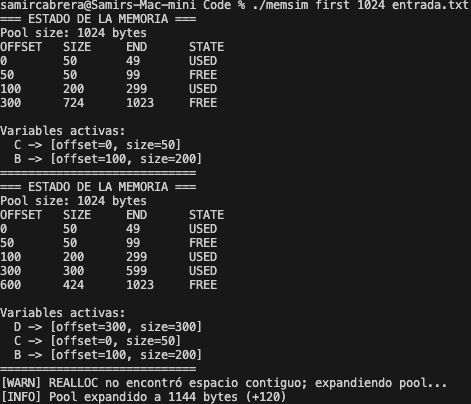
\includegraphics[width=0.9\textwidth]{img/test_first_fit.png.jpeg}
    \caption{Ejecución del simulador con estrategia First-Fit (pool inicial: 1024 bytes)}
    \label{fig:test_first}
\end{figure}

\textbf{Análisis del primer estado (fragmentación):}

El primer estado del sistema muestra claramente el fenómeno de fragmentación externa. Después de liberar la variable A (originalmente de 100 bytes en el offset 0) y asignar la variable C de 50 bytes, se observa:

\begin{itemize}
    \item Bloque USADO en offset 0-49 (50 bytes) - Variable C
    \item Bloque LIBRE en offset 50-99 (50 bytes) - Fragmento residual
    \item Bloque USADO en offset 100-299 (200 bytes) - Variable B
    \item Bloque LIBRE en offset 300-1023 (724 bytes) - Espacio disponible
\end{itemize}

Este estado ilustra perfectamente la fragmentación: existe un bloque libre de 50 bytes que, aunque disponible, está "atrapado" entre bloques ocupados y podría no ser útil para asignaciones futuras de mayor tamaño.

\textbf{Análisis del segundo estado (fuga de memoria):}

Después de asignar las variables D y E, y liberar únicamente E, el sistema muestra:

\begin{itemize}
    \item Variables C (50 bytes), B (200 bytes) y D (300 bytes) permanecen asignadas
    \item El fragmento de 50 bytes persiste en offset 50-99
    \item Espacio libre al final: 424 bytes
\end{itemize}

La variable D representa una fuga de memoria simulada: fue asignada pero nunca liberada, consumiendo 300 bytes que ya no son accesibles pero tampoco están disponibles para el sistema.

\textbf{Comportamiento de expansión:}

Al intentar realizar REALLOC de B de 200 a 260 bytes, First-Fit encuentra que:
\begin{itemize}
    \item No hay espacio contiguo suficiente después del bloque de B (el siguiente bloque es D)
    \item El sistema emite una advertencia y expande el pool
    \item El pool crece de 1024 a 1144 bytes (+120 bytes)
    \item La variable B debe ser reubicada en el nuevo espacio
\end{itemize}

\textbf{Características observadas de First-Fit:}
\begin{itemize}
    \item Velocidad: Las asignaciones son rápidas al detenerse en el primer bloque adecuado
    \item Fragmentación: Tiende a acumular pequeños fragmentos al inicio del pool
    \item Eficiencia espacial: Moderada, con desperdicio en fragmentos pequeños
\end{itemize}

\subsection{Prueba 2: Estrategia Best-Fit}

La segunda prueba ejecuta el simulador con la estrategia Best-Fit sobre un pool inicial más grande de 2048 bytes.

\begin{figure}[H]
    \centering
    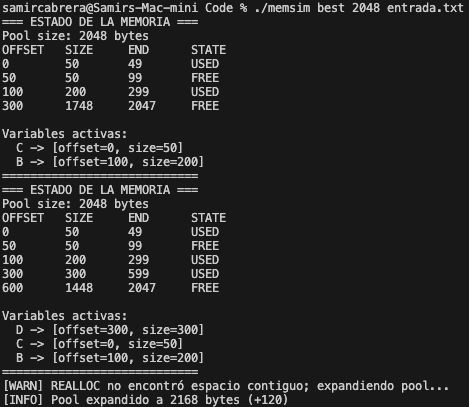
\includegraphics[width=0.9\textwidth]{img/test_best_fit.png.jpeg}
    \caption{Ejecución del simulador con estrategia Best-Fit (test_worst_fit.png inicial: 2048 bytes)}
    \label{fig:test_best}
\end{figure}

\textbf{Análisis del primer estado:}

Con un pool inicial mayor, Best-Fit muestra un comportamiento similar en cuanto a fragmentación:

\begin{itemize}
    \item Fragmento libre de 50 bytes en offset 50-99
    \item Variables C (50 bytes) y B (200 bytes) ocupan las mismas posiciones que en First-Fit
    \item Espacio libre final significativamente mayor: 1748 bytes (vs 724 en First-Fit)
\end{itemize}

La similitud en los primeros bloques es esperada: para estas asignaciones iniciales, Best-Fit coincide con First-Fit porque los primeros bloques disponibles son también los más pequeños adecuados.

\textbf{Diferencias en comportamiento:}

Aunque el patrón de asignación es similar a First-Fit, Best-Fit:
\begin{itemize}
    \item Busca el bloque más ajustado para cada asignación
    \item Minimiza el desperdicio en cada operación individual
    \item Recorre toda la lista de bloques antes de decidir (más lento)
\end{itemize}

\textbf{Expansión del pool:}

Similar a First-Fit, al intentar REALLOC de B a 260 bytes:
\begin{itemize}
    \item No encuentra espacio contiguo adecuado
    \item Expande el pool de 2048 a 2168 bytes (+120 bytes)
    \item Reubica la variable B en el nuevo espacio
\end{itemize}

A pesar de tener el doble de memoria inicial (2048 vs 1024), el problema de espacio contiguo persiste debido a que D está inmediatamente después de B, bloqueando la expansión in-situ.

\textbf{Características observadas de Best-Fit:}
\begin{itemize}
    \item Eficiencia espacial: Mejor aprovechamiento teórico del espacio
    \item Velocidad: Más lenta que First-Fit por recorrer toda la lista
    \item Fragmentación: Genera fragmentos más pequeños y numerosos
    \item Comportamiento similar a First-Fit en este caso particular
\end{itemize}

\subsection{Prueba 3: Estrategia Worst-Fit}

La tercera prueba ejecuta el simulador con la estrategia Worst-Fit sobre un pool inicial reducido de 512 bytes.

\begin{figure}[H]
    \centering
    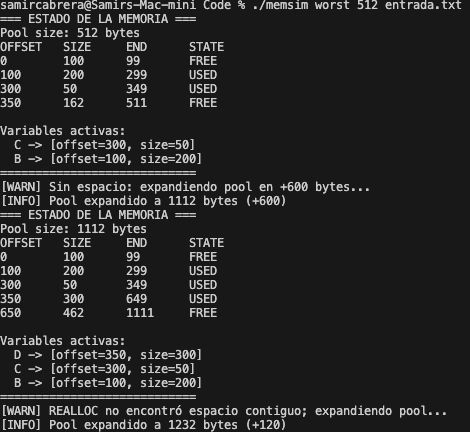
\includegraphics[width=0.9\textwidth]{img/test_worst_fit.png.jpeg}
    \caption{Ejecución del simulador con estrategia Worst-Fit (pool inicial: 512 bytes)}
    \label{fig:test_worst}
\end{figure}

\textbf{Comportamiento diferenciado desde el inicio:}

Worst-Fit muestra un comportamiento notablemente diferente a las otras estrategias:

\begin{itemize}
    \item Bloque LIBRE en offset 0-99 (100 bytes) - Fragmento de A liberado
    \item Bloque USADO en offset 100-299 (200 bytes) - Variable B
    \item Bloque USADO en offset 300-349 (50 bytes) - Variable C
    \item Bloque LIBRE en offset 350-511 (162 bytes)
\end{itemize}

\textbf{Diferencia clave:} Mientras First-Fit y Best-Fit colocaron C al inicio (offset 0), Worst-Fit la colocó cerca del final (offset 300). Esto se debe a que Worst-Fit:
\begin{enumerate}
    \item Después de liberar A, tiene dos bloques libres: uno de 100 bytes (offset 0) y uno grande al final
    \item Al asignar C (50 bytes), selecciona el bloque MÁS GRANDE disponible
    \item Coloca C al final y deja un fragmento residual de 162 bytes
    \item El bloque de 100 bytes al inicio queda completamente libre
\end{enumerate}

\textbf{Primera expansión (asignación de D):}

Con un pool inicial de solo 512 bytes, Worst-Fit enfrenta falta de espacio antes:
\begin{itemize}
    \item Intenta asignar D (300 bytes)
    \item No hay ningún bloque libre de 300 bytes (solo 100 y 162)
    \item El sistema expande agresivamente: +600 bytes (1.17x el tamaño original)
    \item Pool crece de 512 a 1112 bytes
    \item D se asigna en offset 350-649 (inmediatamente después de C)
\end{itemize}

\textbf{Segunda expansión (REALLOC de B):}

Al igual que las otras estrategias, el REALLOC de B requiere expansión:
\begin{itemize}
    \item B debe crecer de 200 a 260 bytes
    \item El siguiente bloque es C (no libre), impidiendo expansión in-situ
    \item Pool expande de 1112 a 1232 bytes (+120 bytes)
\end{itemize}

\textbf{Características observadas de Worst-Fit:}
\begin{itemize}
    \item Distribución diferente: Coloca bloques pequeños en espacios grandes
    \item Fragmentos residuales más grandes: 100 y 162 bytes (vs 50 en otras estrategias)
    \item Expansiones más tempranas: Pool pequeño se agota más rápido
    \item Mayor crecimiento acumulado: 512 → 1232 bytes (2.4x) vs 1024 → 1144 (1.1x) en First-Fit
\end{itemize}

% -------- CONCLUSIONES --------
\section{Conclusiones}

\begin{enumerate}
    \item Se implementó exitosamente un simulador completo de gestión dinámica de memoria que replica el comportamiento de las funciones estándar de C.
    
    \item Las tres estrategias de asignación (First-Fit, Best-Fit, Worst-Fit) fueron implementadas y probadas, demostrando sus características distintivas en términos de velocidad y fragmentación.
    
    \item Se logró demostrar problemas reales de gestión de memoria:
    \begin{itemize}
        \item Fragmentación externa mediante asignaciones y liberaciones intercaladas.
        \item Fugas de memoria dejando variables sin liberar intencionalmente.
    \end{itemize}
    
    \item La expansión dinámica del pool usando \texttt{realloc} permite que el simulador se adapte a cargas de trabajo variables sin fallar por falta de espacio.
    
    \item La coalescencia automática de bloques libres adyacentes mejora significativamente la eficiencia del sistema al reducir la fragmentación.
    
    \item La arquitectura modular del código facilita el mantenimiento, testing y extensión del simulador con nuevas funcionalidades.
    
    \item El proyecto proporciona una comprensión práctica profunda de cómo los sistemas operativos reales gestionan la memoria dinámica, más allá de la abstracción que ofrecen las funciones estándar.
\end{enumerate}

\end{document}